%!TEX root=document.tex


\techreport{\stitle{SeeDB Client}:
\label{sec:SeeDB_frontend}
\SeeDB\ implements a light-weight client that performs two main functions: it
allows the user to select data of interest by issuing a query, 
and it displays recommended visualizations generated from the high-utility views 
returned by the \SeeDB\ backend.
The \SeeDB\ client provides the user three mechanisms for specifying an input query: 
(a) directly filling in SQL into a text box, 
(b) using a query builder tool that allows users
unfamiliar with SQL to formulate queries through a form-based interface, and (c)
using pre-defined query templates which encode commonly performed operations,
e.g., selecting outliers in a particular column. 
Once the user issues a query via the \SeeDB\ client, the backend
evaluates various views and delivers high-utility views to the frontend.
For each view delivered by the backend, the frontend creates and displays the 
corresponding visualization.
Figure~\ref{fig:frontend1} shows a screenshot of the \SeeDB\ frontend showing
the query builder and resulting visualizations in action.}

% To provide a proxy for the visualization software environment, 
%To provide the analyst maximum flexibility in issuing queries, 
%We find that pre-defined query
%templates are particularly useful since analysts are often interested in
%anomalous data points.

% based on parameters such as the data
% type (e.g. ordinal, numeric), number of distinct values, and basic semantics (e.g.
% geography vs. time series).
% The resulting set of visualizations is displayed to the user who can then
% easily examine these $k$ (user-specified) ``most interesting'' visualizations
% at a glance.
% In a full-fledged visualization system, the user would then be able to explore 
% specific views in detail via drill-downs, and study metadata for each view 
% (e.g. size of result, sample data, value with maximum change and other statistics)
% and perform further analysis. \mpv{do we need the screen shot now, might save space. 
% Perhaps link to seedb website?}
%The analyst can also slice-and-dice views further by performing drill-downs on
%specific attributes in the view. 

 
\begin{figure}[htb]
\centerline{
\hbox{\resizebox{9cm}{!}{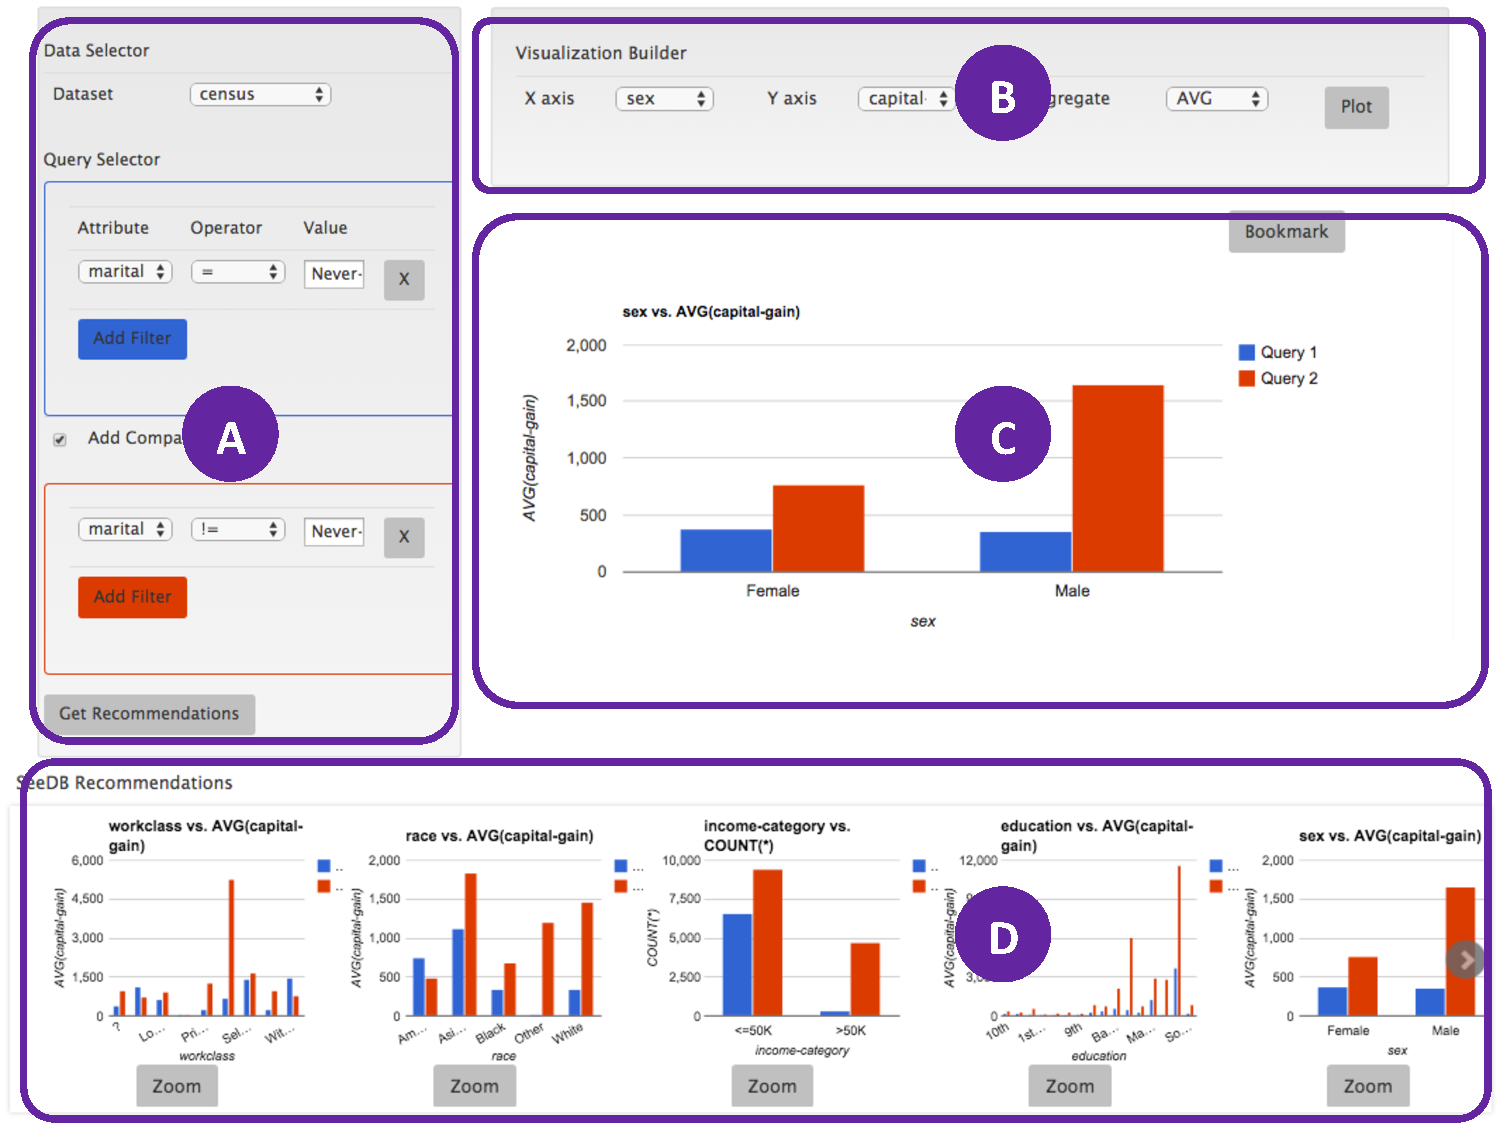
\includegraphics[trim=0mm 0mm 0mm 0mm,
clip=true]{Images/seedb_frontend.pdf}}}}
\caption{\SeeDB Frontend}
\label{fig:frontend1}
\end{figure} 

\reviewer{Update frontend picture and larger description}

%In this work, we focus on the \SeeDB\ backend and develop techniques to
%speed up identification of interesting views. As a result, we leave the
%development of a more advanced and flexible \SeeDB\ frontend for future work. 
% In the next section, we describe the \SeeDB\ execution engine and discuss
% two implementations in detail.
